% Options for packages loaded elsewhere
\PassOptionsToPackage{unicode}{hyperref}
\PassOptionsToPackage{hyphens}{url}
\PassOptionsToPackage{dvipsnames,svgnames,x11names}{xcolor}
%
\documentclass[
  letterpaper,
  DIV=11,
  numbers=noendperiod]{scrartcl}

\usepackage{amsmath,amssymb}
\usepackage{iftex}
\ifPDFTeX
  \usepackage[T1]{fontenc}
  \usepackage[utf8]{inputenc}
  \usepackage{textcomp} % provide euro and other symbols
\else % if luatex or xetex
  \usepackage{unicode-math}
  \defaultfontfeatures{Scale=MatchLowercase}
  \defaultfontfeatures[\rmfamily]{Ligatures=TeX,Scale=1}
\fi
\usepackage{lmodern}
\ifPDFTeX\else  
    % xetex/luatex font selection
\fi
% Use upquote if available, for straight quotes in verbatim environments
\IfFileExists{upquote.sty}{\usepackage{upquote}}{}
\IfFileExists{microtype.sty}{% use microtype if available
  \usepackage[]{microtype}
  \UseMicrotypeSet[protrusion]{basicmath} % disable protrusion for tt fonts
}{}
\makeatletter
\@ifundefined{KOMAClassName}{% if non-KOMA class
  \IfFileExists{parskip.sty}{%
    \usepackage{parskip}
  }{% else
    \setlength{\parindent}{0pt}
    \setlength{\parskip}{6pt plus 2pt minus 1pt}}
}{% if KOMA class
  \KOMAoptions{parskip=half}}
\makeatother
\usepackage{xcolor}
\usepackage[top=1in,left=1in,right=1in,bottom=1in]{geometry}
\setlength{\emergencystretch}{3em} % prevent overfull lines
\setcounter{secnumdepth}{-\maxdimen} % remove section numbering
% Make \paragraph and \subparagraph free-standing
\ifx\paragraph\undefined\else
  \let\oldparagraph\paragraph
  \renewcommand{\paragraph}[1]{\oldparagraph{#1}\mbox{}}
\fi
\ifx\subparagraph\undefined\else
  \let\oldsubparagraph\subparagraph
  \renewcommand{\subparagraph}[1]{\oldsubparagraph{#1}\mbox{}}
\fi

\usepackage{color}
\usepackage{fancyvrb}
\newcommand{\VerbBar}{|}
\newcommand{\VERB}{\Verb[commandchars=\\\{\}]}
\DefineVerbatimEnvironment{Highlighting}{Verbatim}{commandchars=\\\{\}}
% Add ',fontsize=\small' for more characters per line
\usepackage{framed}
\definecolor{shadecolor}{RGB}{241,243,245}
\newenvironment{Shaded}{\begin{snugshade}}{\end{snugshade}}
\newcommand{\AlertTok}[1]{\textcolor[rgb]{0.68,0.00,0.00}{#1}}
\newcommand{\AnnotationTok}[1]{\textcolor[rgb]{0.37,0.37,0.37}{#1}}
\newcommand{\AttributeTok}[1]{\textcolor[rgb]{0.40,0.45,0.13}{#1}}
\newcommand{\BaseNTok}[1]{\textcolor[rgb]{0.68,0.00,0.00}{#1}}
\newcommand{\BuiltInTok}[1]{\textcolor[rgb]{0.00,0.23,0.31}{#1}}
\newcommand{\CharTok}[1]{\textcolor[rgb]{0.13,0.47,0.30}{#1}}
\newcommand{\CommentTok}[1]{\textcolor[rgb]{0.37,0.37,0.37}{#1}}
\newcommand{\CommentVarTok}[1]{\textcolor[rgb]{0.37,0.37,0.37}{\textit{#1}}}
\newcommand{\ConstantTok}[1]{\textcolor[rgb]{0.56,0.35,0.01}{#1}}
\newcommand{\ControlFlowTok}[1]{\textcolor[rgb]{0.00,0.23,0.31}{#1}}
\newcommand{\DataTypeTok}[1]{\textcolor[rgb]{0.68,0.00,0.00}{#1}}
\newcommand{\DecValTok}[1]{\textcolor[rgb]{0.68,0.00,0.00}{#1}}
\newcommand{\DocumentationTok}[1]{\textcolor[rgb]{0.37,0.37,0.37}{\textit{#1}}}
\newcommand{\ErrorTok}[1]{\textcolor[rgb]{0.68,0.00,0.00}{#1}}
\newcommand{\ExtensionTok}[1]{\textcolor[rgb]{0.00,0.23,0.31}{#1}}
\newcommand{\FloatTok}[1]{\textcolor[rgb]{0.68,0.00,0.00}{#1}}
\newcommand{\FunctionTok}[1]{\textcolor[rgb]{0.28,0.35,0.67}{#1}}
\newcommand{\ImportTok}[1]{\textcolor[rgb]{0.00,0.46,0.62}{#1}}
\newcommand{\InformationTok}[1]{\textcolor[rgb]{0.37,0.37,0.37}{#1}}
\newcommand{\KeywordTok}[1]{\textcolor[rgb]{0.00,0.23,0.31}{#1}}
\newcommand{\NormalTok}[1]{\textcolor[rgb]{0.00,0.23,0.31}{#1}}
\newcommand{\OperatorTok}[1]{\textcolor[rgb]{0.37,0.37,0.37}{#1}}
\newcommand{\OtherTok}[1]{\textcolor[rgb]{0.00,0.23,0.31}{#1}}
\newcommand{\PreprocessorTok}[1]{\textcolor[rgb]{0.68,0.00,0.00}{#1}}
\newcommand{\RegionMarkerTok}[1]{\textcolor[rgb]{0.00,0.23,0.31}{#1}}
\newcommand{\SpecialCharTok}[1]{\textcolor[rgb]{0.37,0.37,0.37}{#1}}
\newcommand{\SpecialStringTok}[1]{\textcolor[rgb]{0.13,0.47,0.30}{#1}}
\newcommand{\StringTok}[1]{\textcolor[rgb]{0.13,0.47,0.30}{#1}}
\newcommand{\VariableTok}[1]{\textcolor[rgb]{0.07,0.07,0.07}{#1}}
\newcommand{\VerbatimStringTok}[1]{\textcolor[rgb]{0.13,0.47,0.30}{#1}}
\newcommand{\WarningTok}[1]{\textcolor[rgb]{0.37,0.37,0.37}{\textit{#1}}}

\providecommand{\tightlist}{%
  \setlength{\itemsep}{0pt}\setlength{\parskip}{0pt}}\usepackage{longtable,booktabs,array}
\usepackage{calc} % for calculating minipage widths
% Correct order of tables after \paragraph or \subparagraph
\usepackage{etoolbox}
\makeatletter
\patchcmd\longtable{\par}{\if@noskipsec\mbox{}\fi\par}{}{}
\makeatother
% Allow footnotes in longtable head/foot
\IfFileExists{footnotehyper.sty}{\usepackage{footnotehyper}}{\usepackage{footnote}}
\makesavenoteenv{longtable}
\usepackage{graphicx}
\makeatletter
\def\maxwidth{\ifdim\Gin@nat@width>\linewidth\linewidth\else\Gin@nat@width\fi}
\def\maxheight{\ifdim\Gin@nat@height>\textheight\textheight\else\Gin@nat@height\fi}
\makeatother
% Scale images if necessary, so that they will not overflow the page
% margins by default, and it is still possible to overwrite the defaults
% using explicit options in \includegraphics[width, height, ...]{}
\setkeys{Gin}{width=\maxwidth,height=\maxheight,keepaspectratio}
% Set default figure placement to htbp
\makeatletter
\def\fps@figure{htbp}
\makeatother

\usepackage{booktabs}
\usepackage{longtable}
\usepackage{array}
\usepackage{multirow}
\usepackage{wrapfig}
\usepackage{float}
\usepackage{colortbl}
\usepackage{pdflscape}
\usepackage{tabu}
\usepackage{threeparttable}
\usepackage{threeparttablex}
\usepackage[normalem]{ulem}
\usepackage{makecell}
\usepackage{xcolor}
\KOMAoption{captions}{tableheading,figureheading}
\makeatletter
\@ifpackageloaded{caption}{}{\usepackage{caption}}
\AtBeginDocument{%
\ifdefined\contentsname
  \renewcommand*\contentsname{Table of contents}
\else
  \newcommand\contentsname{Table of contents}
\fi
\ifdefined\listfigurename
  \renewcommand*\listfigurename{List of Figures}
\else
  \newcommand\listfigurename{List of Figures}
\fi
\ifdefined\listtablename
  \renewcommand*\listtablename{List of Tables}
\else
  \newcommand\listtablename{List of Tables}
\fi
\ifdefined\figurename
  \renewcommand*\figurename{Figure}
\else
  \newcommand\figurename{Figure}
\fi
\ifdefined\tablename
  \renewcommand*\tablename{Table}
\else
  \newcommand\tablename{Table}
\fi
}
\@ifpackageloaded{float}{}{\usepackage{float}}
\floatstyle{ruled}
\@ifundefined{c@chapter}{\newfloat{codelisting}{h}{lop}}{\newfloat{codelisting}{h}{lop}[chapter]}
\floatname{codelisting}{Listing}
\newcommand*\listoflistings{\listof{codelisting}{List of Listings}}
\makeatother
\makeatletter
\makeatother
\makeatletter
\@ifpackageloaded{caption}{}{\usepackage{caption}}
\@ifpackageloaded{subcaption}{}{\usepackage{subcaption}}
\makeatother
\ifLuaTeX
  \usepackage{selnolig}  % disable illegal ligatures
\fi
\usepackage{bookmark}

\IfFileExists{xurl.sty}{\usepackage{xurl}}{} % add URL line breaks if available
\urlstyle{same} % disable monospaced font for URLs
\hypersetup{
  pdftitle={Recent Customer Shopping Trends},
  pdfauthor={Ava Cascario, Sydney Holt, and Kacie Rohn},
  colorlinks=true,
  linkcolor={blue},
  filecolor={Maroon},
  citecolor={Blue},
  urlcolor={Blue},
  pdfcreator={LaTeX via pandoc}}

\title{Recent Customer Shopping Trends}
\author{Ava Cascario, Sydney Holt, and Kacie Rohn}
\date{2024-12-03}

\begin{document}
\maketitle

\begin{Shaded}
\begin{Highlighting}[]
\CommentTok{\# Load necessary packages {-}{-}{-}{-}}
\FunctionTok{library}\NormalTok{(ggplot2)}
\FunctionTok{library}\NormalTok{(dplyr)}
\FunctionTok{library}\NormalTok{(kableExtra)}
\FunctionTok{library}\NormalTok{(knitr)}
\FunctionTok{library}\NormalTok{(tinytex)}
\CommentTok{\# Load Data {-}{-}{-}{-}}
\NormalTok{shopping\_trends\_raw }\OtherTok{\textless{}{-}} \FunctionTok{read.csv}\NormalTok{(}
  \AttributeTok{file =} \StringTok{"shopping\_trends.csv"}\NormalTok{, }
  \AttributeTok{header =} \ConstantTok{TRUE}\NormalTok{, }
  \AttributeTok{sep =} \StringTok{","}
\NormalTok{)}
\NormalTok{shopping\_trends\_clean }\OtherTok{\textless{}{-}}\NormalTok{ shopping\_trends\_raw }\SpecialCharTok{\%\textgreater{}\%}
  \FunctionTok{rename}\NormalTok{(}
    \AttributeTok{customer\_id =} \StringTok{"Customer.ID"}\NormalTok{, }
    \AttributeTok{age =} \StringTok{"Age"}\NormalTok{, }
    \AttributeTok{gender =} \StringTok{"Gender"}\NormalTok{, }
    \AttributeTok{item\_purchased =} \StringTok{"Item.Purchased"}\NormalTok{, }
    \AttributeTok{category =} \StringTok{"Category"}\NormalTok{, }
    \AttributeTok{purchase\_amount\_usd =} \StringTok{"Purchase.Amount..USD."}\NormalTok{, }
    \AttributeTok{location =} \StringTok{"Location"}\NormalTok{, }
    \AttributeTok{size =} \StringTok{"Size"}\NormalTok{, }
    \AttributeTok{color =} \StringTok{"Color"}\NormalTok{, }
    \AttributeTok{season =} \StringTok{"Season"}\NormalTok{, }
    \AttributeTok{review\_rating =} \StringTok{"Review.Rating"}\NormalTok{, }
    \AttributeTok{subscription\_status =} \StringTok{"Subscription.Status"}\NormalTok{, }
    \AttributeTok{payment\_method =} \StringTok{"Payment.Method"}\NormalTok{, }
    \AttributeTok{shipping\_type =} \StringTok{"Shipping.Type"}\NormalTok{, }
    \AttributeTok{discount\_applied =} \StringTok{"Discount.Applied"}\NormalTok{, }
    \AttributeTok{promo\_code\_used =} \StringTok{"Promo.Code.Used"}\NormalTok{, }
    \AttributeTok{previous\_purchases =} \StringTok{"Previous.Purchases"}\NormalTok{, }
    \AttributeTok{preferred\_payment\_method =} \StringTok{"Preferred.Payment.Method"}\NormalTok{, }
    \AttributeTok{frequency\_of\_purchases =} \StringTok{"Frequency.of.Purchases"}
\NormalTok{  )}

\NormalTok{type\_reviews }\OtherTok{\textless{}{-}}\NormalTok{ shopping\_trends\_clean }\SpecialCharTok{\%\textgreater{}\%}
  \FunctionTok{select}\NormalTok{(}
\NormalTok{    gender, }
\NormalTok{    review\_rating}
\NormalTok{  ) }\SpecialCharTok{\%\textgreater{}\%}
  \FunctionTok{group\_by}\NormalTok{(}
\NormalTok{    gender, }
\NormalTok{    review\_rating}
\NormalTok{  )}
\FunctionTok{ggplot}\NormalTok{(}
  \AttributeTok{data =}\NormalTok{ type\_reviews,}
  \FunctionTok{aes}\NormalTok{(}
    \AttributeTok{x =}\NormalTok{ gender,}
    \AttributeTok{y =}\NormalTok{ review\_rating}
\NormalTok{  )}
\NormalTok{) }\SpecialCharTok{+}
  \FunctionTok{geom\_boxplot}\NormalTok{()}
\NormalTok{shopping\_summary }\OtherTok{\textless{}{-}} \FunctionTok{lm}\NormalTok{(}\AttributeTok{formula =}\NormalTok{ purchase\_amount\_usd }\SpecialCharTok{\textasciitilde{}}\NormalTok{ category, }\AttributeTok{data =}\NormalTok{ shopping\_trends\_clean)}
\NormalTok{shopping\_summary\_model }\OtherTok{\textless{}{-}} \FunctionTok{summary}\NormalTok{(shopping\_summary)}

\NormalTok{shopping\_summary\_model}\SpecialCharTok{$}\NormalTok{coefficients }\SpecialCharTok{\%\textgreater{}\%}
  \FunctionTok{kable}\NormalTok{() }\SpecialCharTok{\%\textgreater{}\%}
\NormalTok{  kableExtra}\SpecialCharTok{::}\FunctionTok{kable\_classic}\NormalTok{()}
\NormalTok{shopping\_summary }\OtherTok{\textless{}{-}}\NormalTok{ shopping\_trends\_clean }\SpecialCharTok{\%\textgreater{}\%}
  \FunctionTok{select}\NormalTok{(category, purchase\_amount\_usd) }\SpecialCharTok{\%\textgreater{}\%}
  \FunctionTok{group\_by}\NormalTok{(category) }\SpecialCharTok{\%\textgreater{}\%}
  \FunctionTok{summarize}\NormalTok{(}
    \AttributeTok{count =} \FunctionTok{n}\NormalTok{(), }
    \AttributeTok{min =} \FunctionTok{min}\NormalTok{(purchase\_amount\_usd), }
    \AttributeTok{Q1 =} \FunctionTok{quantile}\NormalTok{(purchase\_amount\_usd, }\FloatTok{0.25}\NormalTok{), }
    \AttributeTok{median =} \FunctionTok{median}\NormalTok{(purchase\_amount\_usd), }
    \AttributeTok{Q1 =} \FunctionTok{quantile}\NormalTok{(purchase\_amount\_usd, }\FloatTok{0.75}\NormalTok{), }
    \AttributeTok{max =} \FunctionTok{max}\NormalTok{(purchase\_amount\_usd), }
    \AttributeTok{medianAbsoluteDeviation =} \FunctionTok{mad}\NormalTok{(purchase\_amount\_usd), }
    \AttributeTok{sampleArithmeticMean =} \FunctionTok{mean}\NormalTok{(purchase\_amount\_usd), }
    \AttributeTok{sampleArithmeticSD =} \FunctionTok{sd}\NormalTok{(purchase\_amount\_usd)}
\NormalTok{  )}

\NormalTok{shopping\_summary }\SpecialCharTok{\%\textgreater{}\%}
  \FunctionTok{kable}\NormalTok{() }\SpecialCharTok{\%\textgreater{}\%}
\NormalTok{  kableExtra}\SpecialCharTok{::}\FunctionTok{kable\_classic}\NormalTok{()}
\CommentTok{\# Group data by Location, Season, and Item}
\NormalTok{item\_purchased\_data }\OtherTok{\textless{}{-}}\NormalTok{ shopping\_trends\_clean }\SpecialCharTok{\%\textgreater{}\%}
  \FunctionTok{group\_by}\NormalTok{(}
\NormalTok{    location, }
\NormalTok{    season, }
\NormalTok{    item\_purchased}
\NormalTok{  ) }\SpecialCharTok{\%\textgreater{}\%}
  \FunctionTok{summarize}\NormalTok{(}
    \AttributeTok{item\_count =} \FunctionTok{n}\NormalTok{(), }
    \AttributeTok{.groups =} \StringTok{"drop"}
\NormalTok{  )}
\CommentTok{\# Group States by Region}
\NormalTok{state\_to\_region }\OtherTok{\textless{}{-}} \FunctionTok{c}\NormalTok{(}
  \StringTok{"Maine"} \OtherTok{=} \StringTok{"Northeast"}\NormalTok{, }
  \StringTok{"New Hampshire"} \OtherTok{=} \StringTok{"Northeast"}\NormalTok{, }
  \StringTok{"Vermont"} \OtherTok{=} \StringTok{"Northeast"}\NormalTok{, }
  \StringTok{"Massachusetts"} \OtherTok{=} \StringTok{"Northeast"}\NormalTok{,}
  \StringTok{"Rhode Island"} \OtherTok{=} \StringTok{"Northeast"}\NormalTok{,}
  \StringTok{"Connecticut"} \OtherTok{=} \StringTok{"Northeast"}\NormalTok{,}
  \StringTok{"New York"} \OtherTok{=} \StringTok{"Northeast"}\NormalTok{,}
  \StringTok{"New Jersey"} \OtherTok{=} \StringTok{"Northeast"}\NormalTok{,}
  \StringTok{"Pennsylvania"} \OtherTok{=} \StringTok{"Northeast"}\NormalTok{,}
  \StringTok{"Delaware"} \OtherTok{=} \StringTok{"South"}\NormalTok{,}
  \StringTok{"Maryland"} \OtherTok{=} \StringTok{"South"}\NormalTok{,}
  \StringTok{"Virginia"} \OtherTok{=} \StringTok{"South"}\NormalTok{,}
  \StringTok{"North Carolina"} \OtherTok{=} \StringTok{"South"}\NormalTok{,}
  \StringTok{"South Carolina"} \OtherTok{=} \StringTok{"South"}\NormalTok{,}
  \StringTok{"Georgia"} \OtherTok{=} \StringTok{"South"}\NormalTok{,}
  \StringTok{"Florida"} \OtherTok{=} \StringTok{"South"}\NormalTok{,}
  \StringTok{"West Virginia"} \OtherTok{=} \StringTok{"South"}\NormalTok{,}
  \StringTok{"Kentucky"} \OtherTok{=} \StringTok{"South"}\NormalTok{,}
  \StringTok{"Tennessee"} \OtherTok{=} \StringTok{"South"}\NormalTok{,}
  \StringTok{"Alabama"} \OtherTok{=} \StringTok{"South"}\NormalTok{,}
  \StringTok{"Mississippi"} \OtherTok{=} \StringTok{"South"}\NormalTok{,}
  \StringTok{"Arkansas"} \OtherTok{=} \StringTok{"South"}\NormalTok{,}
  \StringTok{"Louisiana"} \OtherTok{=} \StringTok{"South"}\NormalTok{,}
  \StringTok{"Oklahoma"} \OtherTok{=} \StringTok{"South"}\NormalTok{,}
  \StringTok{"Texas"} \OtherTok{=} \StringTok{"South"}\NormalTok{,}
  \StringTok{"Indiana"} \OtherTok{=} \StringTok{"Midwest"}\NormalTok{, }
  \StringTok{"Illinois"} \OtherTok{=} \StringTok{"Midwest"}\NormalTok{,}
  \StringTok{"Michigan"} \OtherTok{=} \StringTok{"Midwest"}\NormalTok{,}
  \StringTok{"Ohio"} \OtherTok{=} \StringTok{"Midwest"}\NormalTok{,}
  \StringTok{"Wisconsin"} \OtherTok{=} \StringTok{"Midwest"}\NormalTok{,}
  \StringTok{"Missouri"} \OtherTok{=} \StringTok{"Midwest"}\NormalTok{,}
  \StringTok{"Iowa"} \OtherTok{=} \StringTok{"Midwest"}\NormalTok{,}
  \StringTok{"Minnesota"} \OtherTok{=} \StringTok{"Midwest"}\NormalTok{,}
  \StringTok{"North Dakota"} \OtherTok{=} \StringTok{"Midwest"}\NormalTok{,}
  \StringTok{"South Dakota"} \OtherTok{=} \StringTok{"Midwest"}\NormalTok{,}
  \StringTok{"Nebraska"} \OtherTok{=} \StringTok{"Midwest"}\NormalTok{,}
  \StringTok{"Kansas"} \OtherTok{=} \StringTok{"Midwest"}\NormalTok{,}
  \StringTok{"Montana"} \OtherTok{=} \StringTok{"West"}\NormalTok{,}
  \StringTok{"Wyoming"} \OtherTok{=} \StringTok{"West"}\NormalTok{,}
  \StringTok{"Colorado"} \OtherTok{=} \StringTok{"West"}\NormalTok{,}
  \StringTok{"Idaho"} \OtherTok{=} \StringTok{"West"}\NormalTok{,}
  \StringTok{"Nevada"} \OtherTok{=} \StringTok{"West"}\NormalTok{,}
  \StringTok{"Utah"} \OtherTok{=} \StringTok{"West"}\NormalTok{,}
  \StringTok{"Arizona"} \OtherTok{=} \StringTok{"West"}\NormalTok{,}
  \StringTok{"New Mexico"} \OtherTok{=} \StringTok{"West"}\NormalTok{,}
  \StringTok{"Washington"} \OtherTok{=} \StringTok{"West"}\NormalTok{,}
  \StringTok{"Oregon"} \OtherTok{=} \StringTok{"West"}\NormalTok{,}
  \StringTok{"California"} \OtherTok{=} \StringTok{"West"}\NormalTok{,}
  \StringTok{"Alaska"} \OtherTok{=} \StringTok{"West"}\NormalTok{,}
  \StringTok{"Hawaii"} \OtherTok{=} \StringTok{"West"}
\NormalTok{)}
\CommentTok{\# New Column Added for Region}
\NormalTok{item\_purchased\_data }\OtherTok{\textless{}{-}}\NormalTok{ item\_purchased\_data }\SpecialCharTok{\%\textgreater{}\%}
  \FunctionTok{mutate}\NormalTok{(}
    \AttributeTok{region =}\NormalTok{ state\_to\_region[location]}
\NormalTok{  )}
\CommentTok{\# Filter Data by Season}
\NormalTok{spring\_data }\OtherTok{\textless{}{-}}\NormalTok{ item\_purchased\_data }\SpecialCharTok{\%\textgreater{}\%}
  \FunctionTok{filter}\NormalTok{(season }\SpecialCharTok{==} \StringTok{"Spring"}\NormalTok{)}

\NormalTok{summer\_data }\OtherTok{\textless{}{-}}\NormalTok{ item\_purchased\_data }\SpecialCharTok{\%\textgreater{}\%}
  \FunctionTok{filter}\NormalTok{(season }\SpecialCharTok{==} \StringTok{"Summer"}\NormalTok{)}

\NormalTok{fall\_data }\OtherTok{\textless{}{-}}\NormalTok{ item\_purchased\_data }\SpecialCharTok{\%\textgreater{}\%}
  \FunctionTok{filter}\NormalTok{(season }\SpecialCharTok{==} \StringTok{"Fall"}\NormalTok{)}

\NormalTok{winter\_data }\OtherTok{\textless{}{-}}\NormalTok{ item\_purchased\_data }\SpecialCharTok{\%\textgreater{}\%}
  \FunctionTok{filter}\NormalTok{(season }\SpecialCharTok{==} \StringTok{"Winter"}\NormalTok{)}
\CommentTok{\# Visualization of Data by Region Summarized by Season}
\NormalTok{plot\_items\_by\_season }\OtherTok{\textless{}{-}} \ControlFlowTok{function}\NormalTok{(}
\NormalTok{    item\_purchased\_data, }
\NormalTok{    season\_name}
\NormalTok{    ) \{}
\FunctionTok{ggplot}\NormalTok{(}
\NormalTok{  item\_purchased\_data, }
  \FunctionTok{aes}\NormalTok{(}
    \AttributeTok{x =}\NormalTok{ item\_purchased,}
    \AttributeTok{y =}\NormalTok{ item\_count, }
    \AttributeTok{fill =}\NormalTok{ region}
\NormalTok{  )}
\NormalTok{) }\SpecialCharTok{+}
  \FunctionTok{geom\_bar}\NormalTok{(}
    \AttributeTok{stat =} \StringTok{"Identity"}\NormalTok{, }
    \AttributeTok{position =} \FunctionTok{position\_dodge}\NormalTok{(}\AttributeTok{width =} \FloatTok{0.8}\NormalTok{), }
    \AttributeTok{width =} \FloatTok{0.6}
\NormalTok{  ) }\SpecialCharTok{+}
  \FunctionTok{scale\_x\_discrete}\NormalTok{(}
    \AttributeTok{expand =} \FunctionTok{expansion}\NormalTok{(}\AttributeTok{add =} \FunctionTok{c}\NormalTok{(}\FloatTok{0.5}\NormalTok{, }\FloatTok{0.5}\NormalTok{))}
\NormalTok{  ) }\SpecialCharTok{+}
  \FunctionTok{labs}\NormalTok{(}
    \AttributeTok{title =} \FunctionTok{paste}\NormalTok{(}
      \StringTok{"Items Bought by Region"}\NormalTok{, }
\NormalTok{      season\_name}
\NormalTok{    ),  }
    \AttributeTok{x =} \StringTok{"Item"}\NormalTok{, }
    \AttributeTok{y =} \StringTok{"Number of Items Bought"}\NormalTok{, }
    \AttributeTok{fill =} \StringTok{"Region"}
\NormalTok{  ) }\SpecialCharTok{+}
  \FunctionTok{scale\_fill\_manual}\NormalTok{(}
    \AttributeTok{values =} \FunctionTok{c}\NormalTok{(}
      \StringTok{"Northeast"} \OtherTok{=} \StringTok{"\#8DA0CB"}\NormalTok{, }
      \StringTok{"South"} \OtherTok{=} \StringTok{"\#FC8D62"}\NormalTok{, }
      \StringTok{"Midwest"} \OtherTok{=} \StringTok{"\#66C2A5"}\NormalTok{, }
      \StringTok{"West"} \OtherTok{=} \StringTok{"\#E78AC3"}
\NormalTok{    )}
\NormalTok{  ) }\SpecialCharTok{+}
  \FunctionTok{theme\_minimal}\NormalTok{(}\AttributeTok{base\_size =} \DecValTok{14}\NormalTok{) }\SpecialCharTok{+}
  \FunctionTok{theme}\NormalTok{(}
    \AttributeTok{panel.grid.major =} \FunctionTok{element\_blank}\NormalTok{(), }
    \AttributeTok{panel.grid.minor =} \FunctionTok{element\_blank}\NormalTok{(), }
    \AttributeTok{axis.text.x =} \FunctionTok{element\_text}\NormalTok{(}
      \AttributeTok{angle =} \DecValTok{45}\NormalTok{, }
      \AttributeTok{hjust =} \DecValTok{1}\NormalTok{, }
      \AttributeTok{size =} \DecValTok{8}
\NormalTok{    ), }
    \AttributeTok{axis.title.x =} \FunctionTok{element\_text}\NormalTok{(}\AttributeTok{size =} \DecValTok{10}\NormalTok{),}
    \AttributeTok{axis.title.y =} \FunctionTok{element\_text}\NormalTok{(}\AttributeTok{size =} \DecValTok{10}\NormalTok{),}
    \AttributeTok{legend.position =} \StringTok{"top"}\NormalTok{,}
    \AttributeTok{legend.text =} \FunctionTok{element\_text}\NormalTok{(}\AttributeTok{size =} \DecValTok{6}\NormalTok{),}
    \AttributeTok{legend.title =} \FunctionTok{element\_text}\NormalTok{(}\AttributeTok{size =} \DecValTok{8}\NormalTok{), }
    \AttributeTok{legend.key.size =} \FunctionTok{unit}\NormalTok{(}\FloatTok{0.5}\NormalTok{, }\StringTok{"cm"}\NormalTok{),}
    \AttributeTok{plot.title =} \FunctionTok{element\_text}\NormalTok{(}
      \AttributeTok{size =} \DecValTok{16}\NormalTok{, }
      \AttributeTok{hjust =} \FloatTok{0.5}\NormalTok{, }
      \AttributeTok{face =} \StringTok{"bold"}
\NormalTok{    ), }
    \AttributeTok{plot.margin =} \FunctionTok{margin}\NormalTok{(}\DecValTok{15}\NormalTok{, }\DecValTok{15}\NormalTok{, }\DecValTok{15}\NormalTok{, }\DecValTok{15}\NormalTok{)}
\NormalTok{  )}
\NormalTok{\}}
\NormalTok{spring\_plot }\OtherTok{\textless{}{-}} \FunctionTok{plot\_items\_by\_season}\NormalTok{(spring\_data, }\StringTok{"Spring"}\NormalTok{)}
\NormalTok{summer\_plot }\OtherTok{\textless{}{-}} \FunctionTok{plot\_items\_by\_season}\NormalTok{(summer\_data, }\StringTok{"Summer"}\NormalTok{)}
\NormalTok{fall\_plot }\OtherTok{\textless{}{-}} \FunctionTok{plot\_items\_by\_season}\NormalTok{(fall\_data, }\StringTok{"Fall"}\NormalTok{)}
\NormalTok{winter\_plot }\OtherTok{\textless{}{-}} \FunctionTok{plot\_items\_by\_season}\NormalTok{(winter\_data, }\StringTok{"Winter"}\NormalTok{)}

\FunctionTok{print}\NormalTok{(spring\_plot)}
\FunctionTok{print}\NormalTok{(summer\_plot)}
\FunctionTok{print}\NormalTok{(fall\_plot)}
\FunctionTok{print}\NormalTok{(winter\_plot)}
\end{Highlighting}
\end{Shaded}

\section{\texorpdfstring{\textbf{Research Topic: Latest Customer
Shopping
Trends}}{Research Topic: Latest Customer Shopping Trends}}\label{research-topic-latest-customer-shopping-trends}

This research focuses on recent customer shopping trends, a topic that
is both familiar and increasingly important to each member of our team.
The rise of online shopping, particularly after the Covid-19 pandemic,
combined with rapid technological advancements, has made this subject
more relevant than ever. Our research will revolve around gaining a
better understanding on what customers tend to purchase pertaining to
gender, age, geographical location, season, item, price, and other
features.Through a series of research questions and data visualizations,
we will explore these relationships to uncover insights and draw
connections between key attributes. Our goal is to contribute new
knowledge to the reader and deepen our understanding of modern consumer
behavior.

\section{\texorpdfstring{\textbf{Research
Questions}}{Research Questions}}\label{research-questions}

The first research question we will explore is, how do different
demographics such as age, gender, location, and price affect the
shopping trends of customers. We will create different visuals to
present our findings and explain the correlation between each one of
these features and customer shopping behavior. We are also curious to
know, does gender have an affect on how much the customer spends, what
item(s) they buy, and what reviews they left on the product. We predict
that there will be large differences between the shopping trends of
males versus the shopping trends of females, and intend to explore this
further using multiple types of visualizations and tables. We must be
aware of bias, as we are all females who experience the female shopping
trends ourselves, and we cannot allow this to alter the conclusions we
make. We are also curious on if the time of year (season) and
geographical location of a customer changes what specific item they
purchase. For example, does someone who is experiencing summer in
Florida tend to buy something different from a customer experiencing
winter in Maine? Overall, this is not an exhaustive list on what we
intend to explore, as there are many different combinations of features
that allow for different discoveries.

\section{\texorpdfstring{\textbf{Provenance Of Our
Data}}{Provenance Of Our Data}}\label{provenance-of-our-data}

We are utilizing a data set that we found on Kaggle. Kaggle is a website
focused towards data scientists with a goal in helping others learn
about data. The author of the data is Bhadra Mohit, and they describe it
as offering a comprehensive view of consumer shopping trends, aiming to
uncover patterns and behaviors in retail purchasing. It contains
detailed transactional data across various product categories, customer
demographics, and purchase channels. This data set was last updated 20
days ago, and is expected to be updated 4 times a year. This ensures
that the data remains relevant and is as accurate as possible. In this
data set, case is an individual transaction. This includes the
attributes, customer ID, age, gender, item purchased, category, purchase
amount USD, location, size, color, season, review rating, subscription
status, payment method, shipping type, discount applies, promo code
used, previous purchases, preferred payment method, and frequency of
purchases. We intend to focus on age, gender, item purchased, location,
season, review rating, and previous purchases. All of the attributes
come from the data set, but we also created the attribute of region,
which groups all fifty states into four regions: Northeast, South,
Midwest, and West. This is based upon the national recognized regions in
the United States.

\section{\texorpdfstring{\textbf{FAIR
Principles}}{FAIR Principles}}\label{fair-principles}

The data we are utilizing meets the FAIR principles. The data is
\textbf{findable}, and includes unique identifiers as well rich and
substantial metadata. Each case is given an ID number, and there are
numerous attributes that they are defined by. The data is
\textbf{accessible} and can be found in our public repository. We also
downloaded the data from Kaggle, which is public and we were able to
easily locate it and access it. The data is \textbf{interoperable} and
uses the R language which is widely known and accepted. This way our
data can be exchanged between collaborators and allows for open
communication. By citing our sources and explaining the provenance of
our data, this ensure our data is also \textbf{reusable}. By meeting the
FAIR principles we are ensuring that our data is universal, and can be
easily understood.

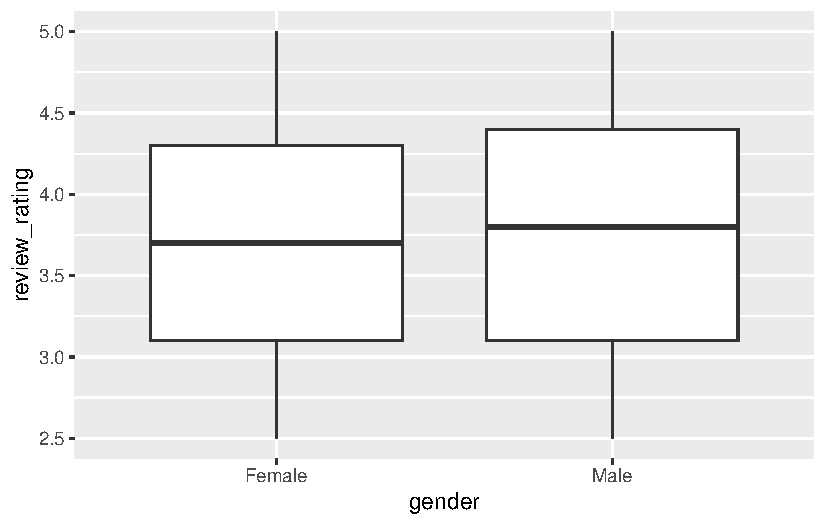
\includegraphics{Quarto-Stat-184-Final-Project_files/figure-pdf/vizualization_for_gender_review-1.pdf}

\begin{longtable*}[t]{lrrrr}
\toprule
 & Estimate & Std. Error & t value & Pr(>\&\#124;t\&\#124;)\\
\midrule
(Intercept) & 59.8387097 & 0.6725026 & 88.9791512 & 0.0000000\\
categoryClothing & 0.1866214 & 0.8804070 & 0.2119717 & 0.8321402\\
categoryFootwear & 0.4167160 & 1.1783422 & 0.3536460 & 0.7236233\\
categoryOuterwear & -2.6658702 & 1.4775420 & -1.8042602 & 0.0712677\\
\bottomrule
\end{longtable*}

\begin{longtable*}[t]{lrrrrrrrr}
\toprule
category & count & min & Q1 & median & max & medianAbsoluteDeviation & sampleArithmeticMean & sampleArithmeticSD\\
\midrule
Accessories & 1240 & 20 & 80 & 60.0 & 100 & 29.6520 & 59.83871 & 23.30123\\
Clothing & 1737 & 20 & 81 & 60.0 & 100 & 31.1346 & 60.02533 & 23.79246\\
Footwear & 599 & 20 & 81 & 60.0 & 100 & 31.1346 & 60.25543 & 23.63844\\
Outerwear & 324 & 20 & 80 & 54.5 & 100 & 33.3585 & 57.17284 & 24.59003\\
\bottomrule
\end{longtable*}

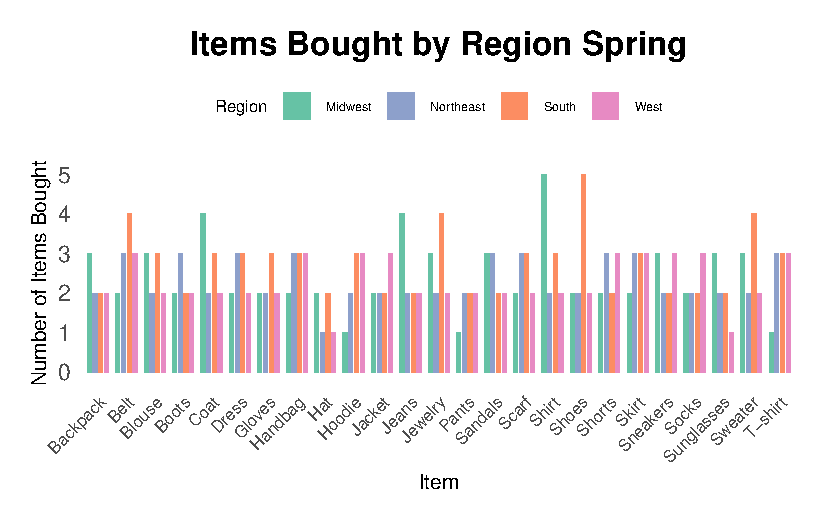
\includegraphics{Quarto-Stat-184-Final-Project_files/figure-pdf/create_each_plot-1.pdf}

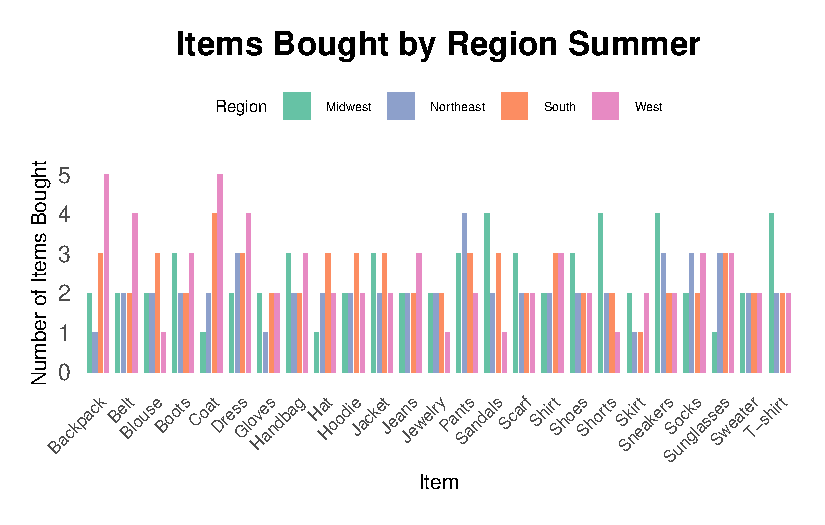
\includegraphics{Quarto-Stat-184-Final-Project_files/figure-pdf/create_each_plot-2.pdf}

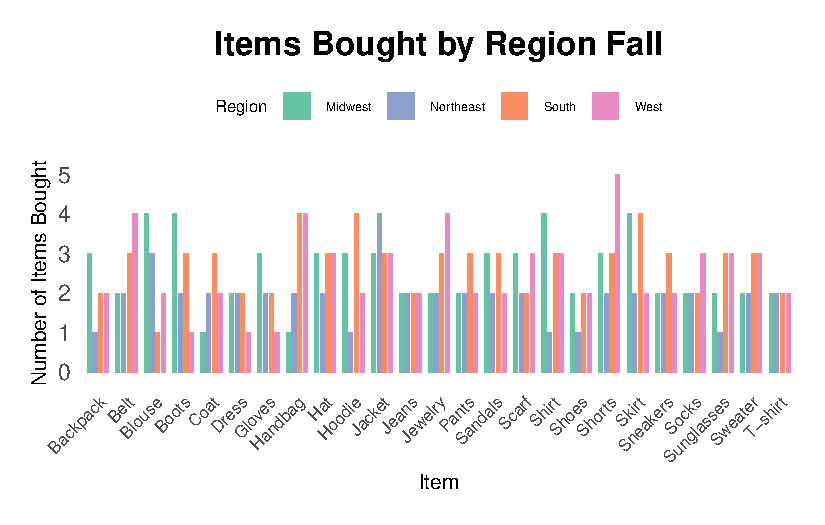
\includegraphics{Quarto-Stat-184-Final-Project_files/figure-pdf/create_each_plot-3.pdf}

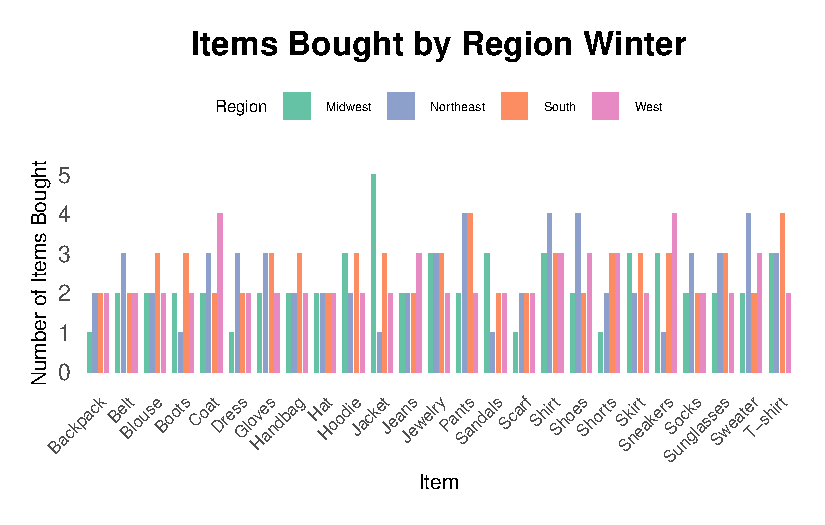
\includegraphics{Quarto-Stat-184-Final-Project_files/figure-pdf/create_each_plot-4.pdf}



\end{document}
